\documentclass[../main]{subfiles}
\begin{document}

\section{Performance evaluation of metacompiling strategies}
\label{lbl:compile-time-eval}

In this section, we observe the impact of the previously introduced techniques
on compiler execution time. We will also assess their implementation costs
by comparing the amount of additional code it takes to generate code from
\constexpr dynamic structures.

To provide more

In this section we observe the impact of metacompiling on compiler execution
time and validate the implementation of metacompilers with different methods.
We first introduce the different methodologies used to benchmark and validate
metacompiler implementations, then proceed with measurements and observations
for the BF metacompiler and the mathematical formula metacompiler.

\subsection{Methodology}

All the benchmarks and tests were run on an i5 6300U with 8GB of RAM, and only
Clang 16.0.6 was used as GCC 12.2.1 lacks support for features used in the
project such as implicit lambda capture of \constexpr variables. The system was
tuned using \lstinline{pyperf} to improve measurement accuracy.
\\

Variable-size benchmarks were made with a toolset developed to declare and run
compile time benchmarks using Clang's built-in profiler, which is used to
measure and plot compiler execution times. It relies on the \cpp pre-processor
to instantiate benchmark cases for each size.
Single time measurements were done using the \lstinline{time} shell command.

\subsection{BF metacompiler evaluation}

\subsubsection{Small variable-size benchmarks}

We first begin by running two variable-sized benchmarks, consisting in
measuring compiler execution time as the AST widens, and as the AST deepens.\\

The first variable-sized benchmark consists in generating a valid BF AST by
concatenating strings to generate a succession of BF while loops in a
\constexpr string. This benchmark was instantiated with sizes going from 1 to
10 with a step of 1, with 10 timing iterations for each size.\\

The second benchmark generates a string with
nested loops, making the AST deeper as the benchmark size increases instead
of making it wider as in the previous case.\\

Both benchmarks generate programs of the same size so comparisons can be made
properly.

\begin{figure}
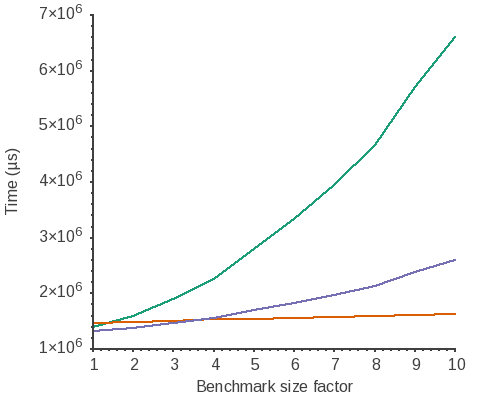
\includegraphics[scale=0.5]{images/bf-consecutive_loops.png}
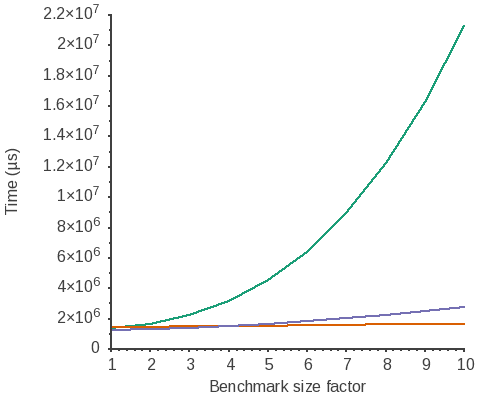
\includegraphics[scale=0.5]{images/bf-imbricated_loops.png}
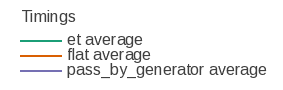
\includegraphics[scale=0.5]{images/bf-graph-legend.png}
\caption{
  Compiler execution time measurements for consecutive loops (left) and nested loops (right)
}\label{fig:bf-bench}
\end{figure}

Figure \ref{fig:bf-bench}
both highlight considerably higher compiler execution times for the expression
template based backend, high enough to suggest that the use of expression
templates induces an overhead higher than parsing and generating BF programs
using the pass-by-generator backend. However the pass-by-generator backend still
has a compile time overhead much higher than the flat backend, which shows near
constant compiler execution times on these small scale benchmarks.\\

Finally, AST deepening has a much higher impact on compile times than AST
widening with the expression template backends, whereas the other backends seem
to scale similarly as the AST grows wider or deeper.

\subsubsection{Realistic BF programs}

The following benchmarks consist in measuring compiler execution times for
compiling BF code examples. These example programs are also used to validate the
metacompiler's backend implementations by compiling them and verifying their
output.

\begin{itemize}
\item A Hello World program (106 tokens).
\item The same Hello World program, ran twice (212 tokens).
\item A Mandelbrot set fractal viewer (11672 tokens).
\end{itemize}

\begin{figure}
\begin{tabular}{|c|c|c|c|}
\hline
Backend             & Hello World & Hello World x2  & Mandelbrot \\
\hline
Flat                & 1.81        & 2.25            & 49.68 \\
Pass-by-generator   & 9.77        & 34.37           & Failure (timeout) \\
Expression template & 50.60       & 192.73          & Failure (timeout) \\
\hline
\end{tabular}
\caption{BF compile time measurements in seconds
}\label{fig:BF-compile-times}
\end{figure}

The measurements in figure~\ref{fig:BF-compile-times} help us better understand
how various metacompiling techniques behave at scale. The "Flat" backend shows
very good performance on all examples, including the Mandelbrot example that is
about 100 times larger than the Hello World example. However the other cases
highlight severe scaling issues and tend to confirm our previous hypothesis
being that using generator functions to pass values makes the code generation
quadratic. Finally, the "Expression template" backend performance highlights
heavy performance impact when expression templates are being used, which is
likely due to the complexity of the mechanisms expression templates involve like
SFINAE and overload resolution.

\subsection{Formula metacompiler evaluation}

The mathematical formula metacompiler uses a slighlty different code generation
technique. It can be used with or without Blaze, and Blaze can be used alone as
well. In this subsection we are therefore measuring compiler execution times for
the metacompiler for code generation using Blaze, but also for code generation
without Blaze by doing simple math operations on integers, and using Blaze
alone.

\subsubsection{Variable-size benchmark cases}

To evaluate the performance compile time impact of mathematical formula parsing,
we run benchmarks for two cases:

\begin{itemize}
\item \lstinline{no-formula-blaze}: Blaze code generation using the library's
      own API, \ie its own \dsel based on \cpp operator overloading.
\item \lstinline{formula-blaze}: Blaze code generation from a formula parsed at
      compile time and transformed into a Blaze expression.
\end{itemize}

Both benchmarks consist in running a series of additions
\lstinline{x + y + ... x} with \lstinline{x + y + } repeated N times, and the
variables \lstinline{x} and \lstinline{y} of type
\lstinline{blaze::DynamicVector<unsigned int>}.

\begin{figure}
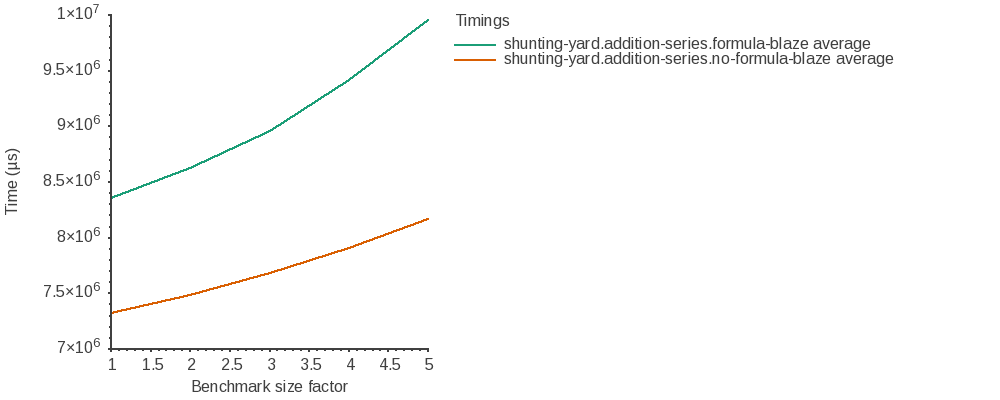
\includegraphics[scale=0.5]{
  images/shunting-yard.addition-series.graph.png
}
\caption{Execution time measurements for math formula compilation
}\label{fig:sy-rubbish-benchmark-graph}
\end{figure}

The figure~\ref{fig:sy-rubbish-benchmark-graph} shows a compiler execution time
overhead of around 20\% when adding compile time parsing.
While it is noticeable, Blaze still accounts for most of the compiler execution
time.

\clearpage%

\end{document}
